% !TeX spellcheck = <none>
\documentclass[10pt,a4paper]{article}
\usepackage[utf8]{inputenc}
\usepackage{amsmath}
\usepackage{amsfonts}
\usepackage{amssymb}
\usepackage{graphicx}
%%% formatting the code
\usepackage{listings}



\usepackage{color}
\lstset{%
	escapeinside={(*}{*)},%
}

\newcommand{\amidstversion}{\input{../../version.txt}}

\lstset{
	frameround=fttt,
%	language=java,
	numbers=left,
	breaklines=true,
	mathescape, 
	columns=fullflexible, 
	basicstyle=\fontfamily{lmvtt}\selectfont,
	keywordstyle=\color{blue}\fontfamily{lmvtt}\selectfont, 
	numberstyle=\color{black}
}
\lstMakeShortInline[columns=fixed]|



\newcommand{\includejavasource}[1]{\lstinputlisting[language=java]{#1}}
\newcommand{\inlinejava}[1]{\lstinline[columns=fixed,language=java]{#1}}

\newcommand{\lang}[1]{}



\usepackage{hyperref}



\begin{document}

\section{Modeling concept drift: A probabilistic graphical model based approach
}\label{sec:blog_conceptdrift}
%\subsection{Introduction}\label{sec:lvmodels:intro}

Here we explain in a simple way how the AMIDST toolbox can be use for detecting the effect of concept drift in the context of big data streams: we informally describe such phenomenon and explain how it can be detected using Bayesian networks with latent variables. Finally, we show some code examples. For further details of this approach, check the following article:

\begin{quotation}
Borchani et al. Modeling concept drift: A probabilistic graphical model based approach. IDA 2015.
\end{quotation}

%\begin{figure}[h!]
%	\centering
%	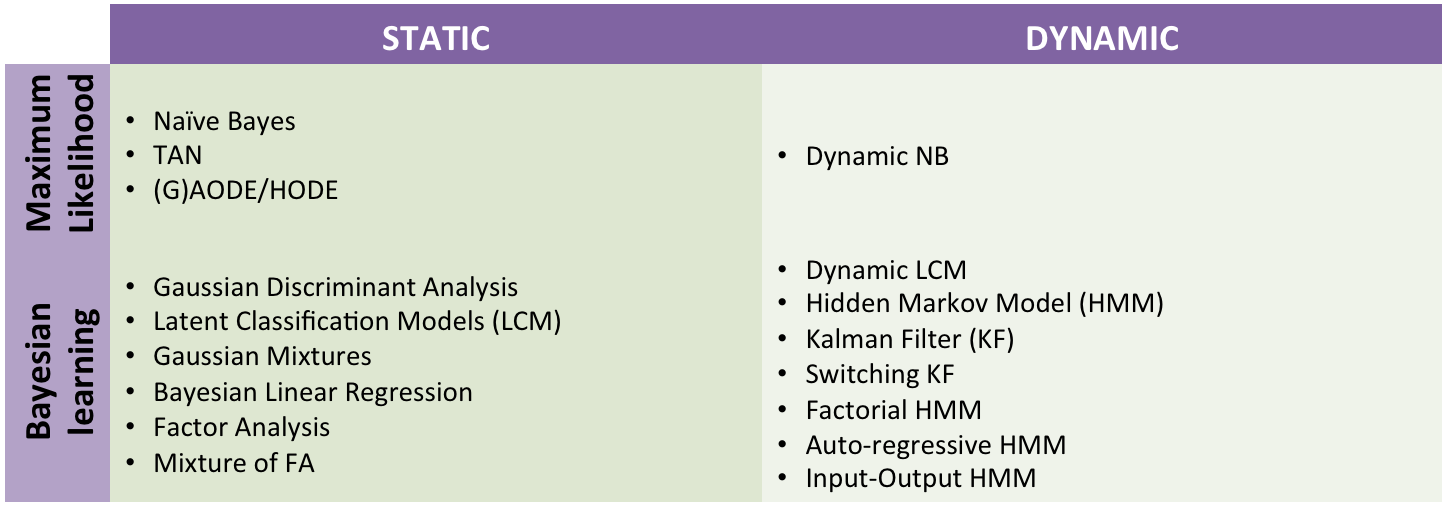
\includegraphics[width=13cm]{img/amidstModels.png}
%	\caption{Set of predefined latent variable models in AMIDST}
%	\label{fig:lvmodels:amidstModels}	
%\end{figure}

\subsection{What is concept drift?}\label{sec:blog_conceptdrift:what}

In non-stationary domains, the distribution governing the data may change over time. This effect is known as concept drift. When doing classification in the context of big data streams, this effect can make the accuracy of our model to drop significantly. As an example, let us consider the image below which shows a naive Bayes classifier for predicting if a particular client of a bank will default in the following months.  

\begin{figure}[h!]
	\centering
	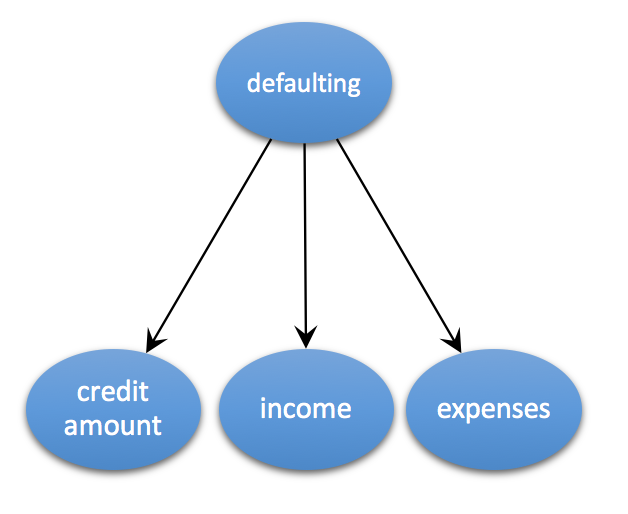
\includegraphics[width=13cm]{img/defaulters_nb.png}
	\caption{Simple naive Bayes classifier for detecting potential defaulters.}
	\label{fig:blog_conceptdrift:what:nb}	
\end{figure}

Previous classifier contains 3 predictive attributes (credit amount, income and expenses) which are continuous variables with Gaussian distributions associated. The class variable is a multinomial (i.e. discrete) variable taking 2 possible values indicating if a given client will default or not.\newline  

The data set used in the learning process, which was provided by Banco de Cr{\'e}dito Cooperativo (BCC), contains monthly aggregated information for a set of clients of BCC for the period from April 2007 to March 2014.  Figure 2 shows the evolution of the variables considered in the classifier. The plots reveal that both seasonal and global trends appear to be present in the data set.

\begin{figure}[h!]
	\centering
	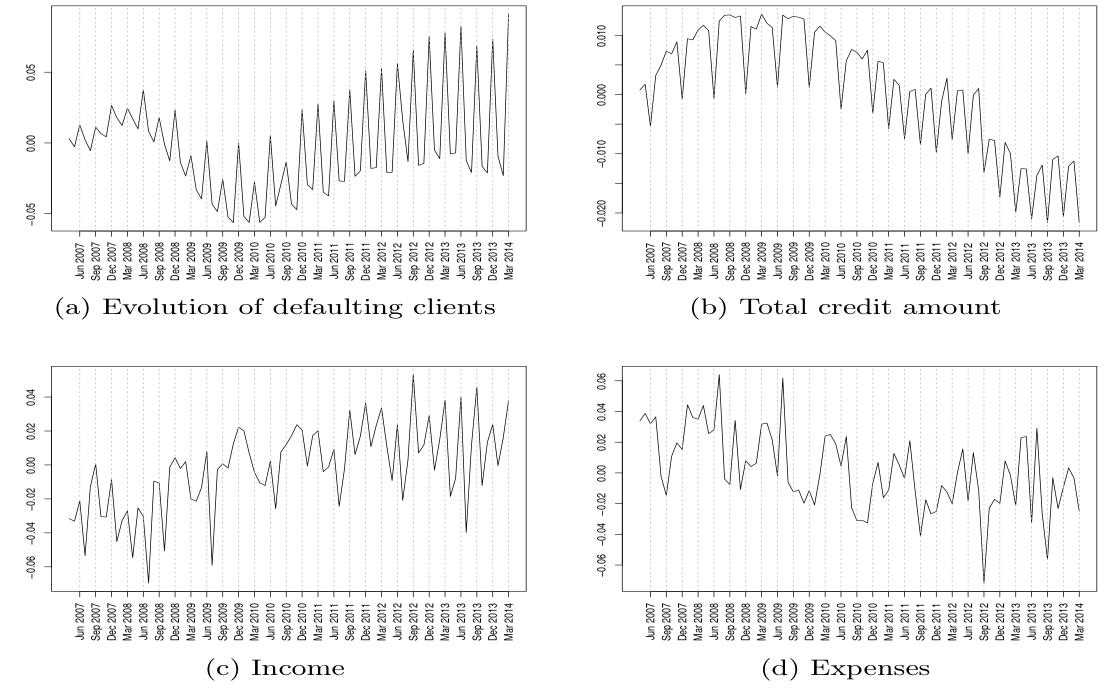
\includegraphics[width=13cm]{img/graphics_cd.png}
	\caption{Evolution of defaulting clients and of the variables considered from the financial data set.}
	\label{fig:blog_conceptdrift:what:graphics_cd}	
\end{figure}



As mentioned before, this variation in the distribution of the data can make the learnt model to offer bad results. One possible solution could be monitoring the accuracy and restart the learning process as son as accuracy drops. However, in those domains where the class variable is highly imbalanced this solution can be misleading. This is the case of previous classifier, where the number of defaulters is small compared to the total number of clients.

In a classification model, concept drift situations can be further classified as either real concept drift, when the probability distribution of the class and the predictive attributes changes with time, or virtual concept drift, when the probability of the attributes drifts while the distribution of the class remains constant. For simplicity, we will only consider the last situation.


\subsection{Model for detecting concept drift}\label{sec:blog_conceptdrift:model}


In our approach, we propose the use of latent (i.e. hidden) variables for the detection of concept drift. Before explaining this approach, we will how the data is structured for its analysis. An instance is a vector containing a value for each variable in the classifier to be analyzed. In our example, each instance is basically the information we have in our records about a client in a given point of time (credit amount, income, expenses, and if he defaulted or not). At each time point we have a collection of instances (also called window or batch). The figure below shows a scheme of this structure. We shall assume that concept drift only happens across time steps and not within a collection of instances captured at the same time-point, i.e., we assume that the distribution of the data does not vary inside a batch.


\begin{figure}[h!]
	\centering
	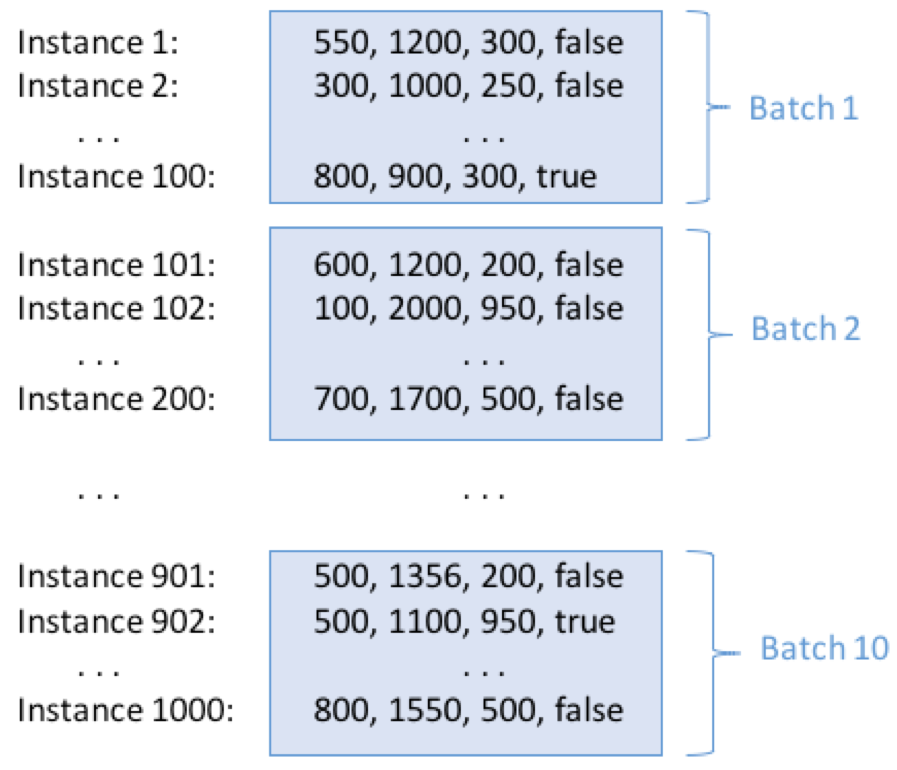
\includegraphics[width=13cm]{img/cd_stream.png}
	\caption{Structure of the stream of data used for learning the simple naive Bayes classifier for detecting potential defaulters.}
	\label{fig:blog_conceptdrift:what:cd_stream}	
\end{figure}


Latent variables are variables that are not directly observed but are rather inferred from other variables that are observed. In our model, we use a latent variable Ht which is parent of the predictive attributes for each batch or instant of time t (see figure below).  Note also that depending on the nature of the variable Ht, this model allows us to represent both gradual (Ht continuous) and abrupt (Ht discrete) concept drift. Furthermore, the model can easily be extended to model multiple concepts drifts by introducing multiple latent variables, each representing a different drift regime.\newline 

\begin{figure}[h!]
	\centering
	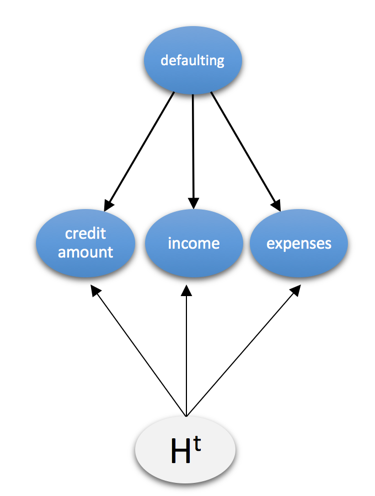
\includegraphics[width=13cm]{img/cd_detector.png}
	\caption{Simple naive Bayes classifier for detecting potential defaulters including a latent variable for detecting concept drift.}
	\label{fig:blog_conceptdrift:what:cd_detector}	
\end{figure}


In previous model, detecting the presence of concept drift simply means learning the distribution associated to each Ht and comparing them. The learning task can be transformed in the inference process of calculating the probability of Ht given all the instances in the instant of time t. This is done as follows: for each instance we create a classifier with all the nodes instantiated with the corresponding values in the instance. Then, an arc from Ht to each attribute predictive in the batch is included. The following figure shows an example of this model.\newline 


\begin{figure}[h!]
	\centering
	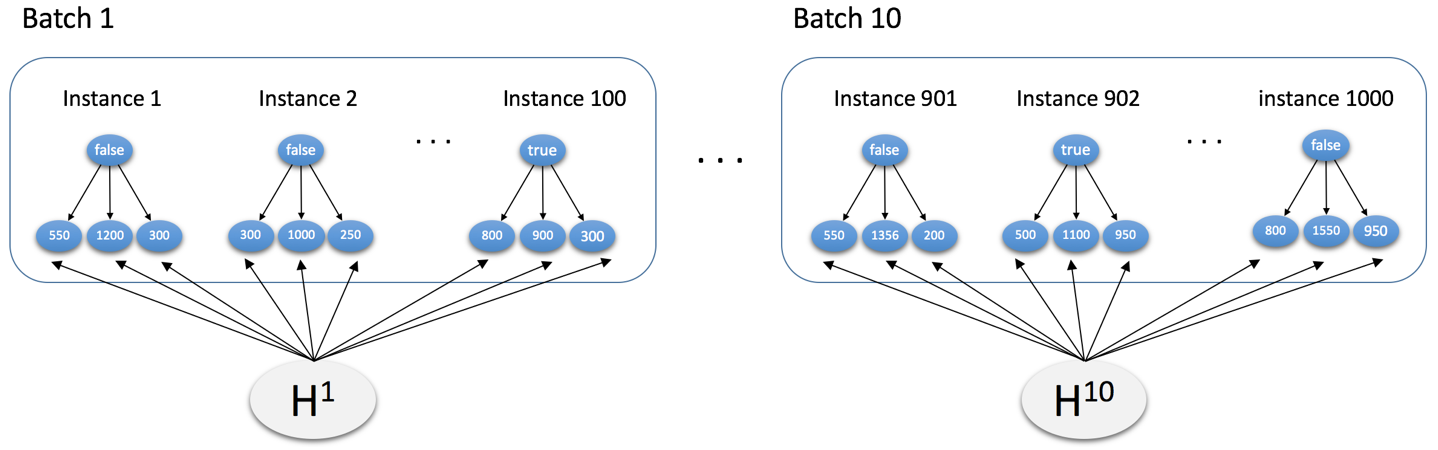
\includegraphics[width=15cm]{img/cd_detector2.png}
	\caption{Model used for learning the distribution of $H$.}
	\label{fig:blog_conceptdrift:what:cd_detector2}	
\end{figure}

In short, to detect the presence of concept drift we just have to compute mean of the Gaussian distribution $P(H^t \vert D^t)$. If such values varies significantly, the conclusion is that the data drifts.\newline 


\subsection{Code Example}\label{sec:blog_conceptdrift:what}

In the following, we show a code example for detecting concept drift in a data stream. A guide for adding the AMIDST library to your project can be found here [add link]. The full code and dataset used can be download here [add link].\newline 

Initially, we open a data stream using the static class \textit{DataStreamLoader}. In this example we will load a data stream from an arff file. Each instance in this data stream contains 3 continuous predictive variables and a discrete class variable.\newline 

\begin{verbatim}
DataStream<DataInstance> data = DataStreamLoader.openFromFile("./datasets/DriftSets/sea.arff");
\end{verbatim}

The class that provides all the functionality related to the detection of concept drift is \textit{NaiveBayesVirtualConceptDriftDetector}. Thus we create an object of such class.

\begin{verbatim}
NaiveBayesVirtualConceptDriftDetector virtualDriftDetector = new NaiveBayesVirtualConceptDriftDetector();
\end{verbatim}




Before any processing, we must set the values for all the parameters of the detector. The method \textit{setClassIndex} is used to indicate the position of the class variable in the stream (e.g the 1st position has the index 1 and so on). The data stream is associated to the detector with the method \textit{setData}. Finally we set the transition variance and the number of hidden variables with the methods \textit{setTransitionVariance} and \textit{setNumberOfGlobalVars}.

\begin{verbatim}
//We set class variable as the last attribute
//We set the data which is going to be used
//We fix the size of the window
//We fix the so-called transition variance
//We fix the number of global latent variables
virtualDriftDetector.setClassIndex(4);
virtualDriftDetector.setData(data);
int windowSize = 1000;
virtualDriftDetector.setWindowsSize(windowSize);
virtualDriftDetector.setTransitionVariance(0.1);
virtualDriftDetector.setNumberOfGlobalVars(1);
\end{verbatim}


Afterwards, we must invoke the method \textit{initLearning}. The we show the graph, including the hidden variable, used for the detection.

\begin{verbatim}
virtualDriftDetector.initLearning();
System.out.println(virtualDriftDetector.getLearntBayesianNetwork().getDAG());
\end{verbatim}


Finally we iterate over the stream. At each iteration, our model is a batch (i.e. a set of instances) is used for updating our model. An important variation in the value returned means that our data drifts.

\begin{verbatim}
for (DataOnMemory<DataInstance> batch : data.iterableOverBatches(windowSize)){
    double[] out = virtualDriftDetector.updateModel(batch);
    System.out.println(out[0]+"\t");
}
\end{verbatim}
\end{document}